\section{Deskriptive Statistik}

\begin{concept}{Teilbereiche der Statistik}
\begin{itemize}
    \item \textbf{Deskriptive Statistik:} Beschreibung und übersichtliche Darstellung von Daten, Ermittlung von Kenngrössen und Datenvalidierung
    \item \textbf{Explorative Statistik:} Weiterführung und Verfeinerung der beschreibenden Statistik, insbesondere die Suche nach Strukturen und Besonderheiten
    \item \textbf{Induktive Statistik:} Versucht mithilfe der Wahrscheinlichkeitsrechnung über die erhobenen Daten hinaus allgemeinere Schlussfolgerungen zu ziehen
\end{itemize}
\end{concept} 

\begin{definition}{Statistische Grundbegriffe}
\begin{itemize}
    \item \textbf{Merkmalsträger/Statistische Einheiten:} Objekte, an denen interessierende Grössen beobachtet und erfasst werden (z.B. Wohnungen, Menschen, Unternehmen)
    \item \textbf{Grundgesamtheit:} Alle statistischen Einheiten, über die man Aussagen gewinnen möchte. Kann endlich oder unendlich, real oder hypothetisch sein
    \item \textbf{Vollerhebung:} Eigenschaften werden bei jedem Individuum in der Grundgesamtheit erhoben
    \item \textbf{Stichprobe:} Untersuchte Teilmenge der Grundgesamtheit, soll diese möglichst genau repräsentieren
    \item \textbf{Stichprobenumfang:} Anzahl der Einheiten in der Stichprobe
    \item \textbf{Urliste:} Liste der beobachteten Stichprobenwerte
    \item \textbf{Merkmal:} Interessierende Grösse, die an den statistischen Einheiten beobachtet wird
    \item \textbf{Merkmalsausprägungen:} Verschiedene Werte, die jedes Merkmal annehmen kann
\end{itemize}
\end{definition}



\raggedcolumns

\begin{concept}{Merkmalstypen}
\begin{itemize}
    \item \textbf{Qualitativ/Kategoriell:} eine Ausprägung, kein Ausmass angegeben
    \begin{itemize}
        \item \textbf{Nominal:} Reine Kategorisierung, keine Ordnung 
        \item \textbf{Ordinal:} Ordnung vorhanden, Rangierung möglich
    \end{itemize}
    \item \textbf{Quantitativ/Metrisch:} Es wird ein Ausmass mit Zahlen angegeben
    \begin{itemize}
        \item \textbf{Diskret:} Endlich viele / abzählbar unendlich viele Ausprägungen
        \item \textbf{Stetig:} Alle Ausprägungen in einem reellen Intervall
    \end{itemize}
\end{itemize}

\begin{center}
    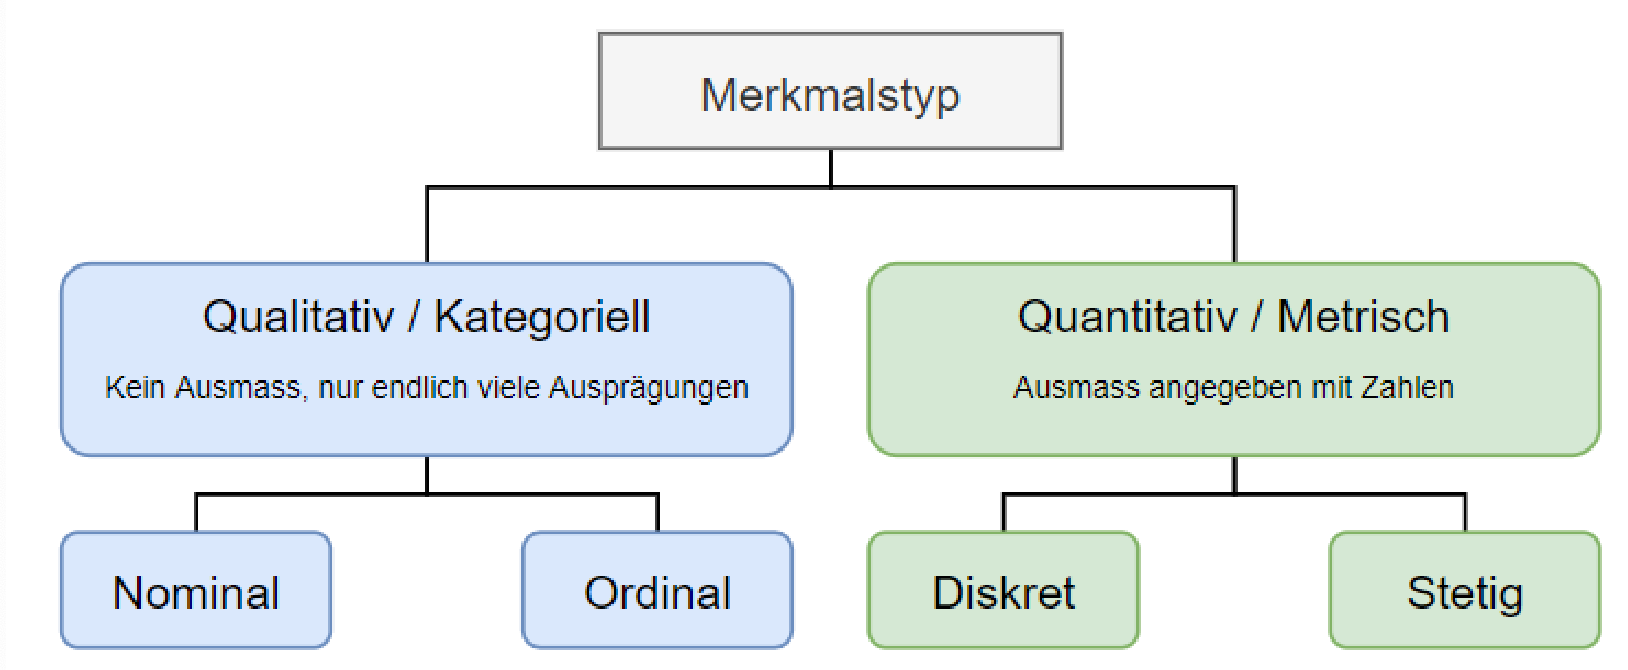
\includegraphics[width=0.8\textwidth]{images/merkmalstypen.png}
\end{center}
\end{concept}

\begin{example2}{Merkmalstypen}
    \small
\begin{itemize}
    \item \textbf{Würfelwurf (4-mal)} Messniveau: Metrisch diskret
    \begin{itemize}
        \item Merkmalsausprägungen: Zahlen 1 bis 6
    \end{itemize}
    
    \item \textbf{Parteiwahl (100 Menschen)} Messniveau: Nominal
    \begin{itemize}
        \item Merkmalsausprägungen: BDP, CVP, FDP, GLP, etc.
    \end{itemize}
    
    \item \textbf{Programmrobustheit (100 Tests)} Messniveau: Ordinal
    \begin{itemize}
        \item Merkmalsausprägungen: schlecht, mittel, sehr gut
    \end{itemize}
    
    \item \textbf{Programmlaufzeit (100 Tests)} Messniveau: Metrisch stetig
    \begin{itemize}
        \item Merkmalsausprägungen: Laufzeiten
    \end{itemize}
\end{itemize}
\end{example2}

\subsection{Häufigkeiten und Verteilungsfunktion}

\subsubsection{Grundlegende Begriffe}

\begin{formula}{Symbole und Bezeichnungen}

    \begin{minipage}[t]{0.5\columnwidth}
        \begin{itemize}
            \item $\Omega =$ Grundgesamtheit
            \item $n =$ Anzahl Objekte\\ (Stichprobenumfang)
            \item $a =$ Ausprägungen
            \item $a_i =$ $i$-te Ausprägung
            \item $m =$ Anzahl verschiedener\\ Merkmalsausprägungen
            \item $d =$ Klassenbreite
        \end{itemize}
    \end{minipage}
    \begin{minipage}[t]{0.5\columnwidth}
        \begin{itemize}
            \item $X =$ Stichprobenwerte
            \item $x =$ Einzelner Stichprobenwert
            \item $h =$ Absolute Häufigkeit
            \item $f =$ Relative Häufigkeit
            \item $H =$ Kumulative Absolute\\ Häufigkeit
            \item $F =$ Kumulative Relative\\ Häufigkeit
        \end{itemize}
    \end{minipage}
    %TODO: Add more symbols    
\end{formula}

\begin{definition}{Grundlegende Unterscheidungen}
\begin{itemize}
    \item \textbf{Diskrete vs. Stetige Merkmale:}
    \begin{itemize}
        \item Diskret: PMF, Höhe = Wahrscheinlichkeit
        \item Stetig: PDF, Fläche = Wahrscheinlichkeit
    \end{itemize}
    \item \textbf{Nicht-klassiert vs. Klassiert:}
    \begin{itemize}
        \item Nicht-klassiert: Einzelwerte
        \item Klassiert: Intervalle mit Häufigkeitsdichten
    \end{itemize}
    \item \textbf{Absolut vs. Relativ:}
    \begin{itemize}
        \item Absolut: Konkrete Anzahlen
        \item Relativ: Anteile (durch n geteilt)
    \end{itemize}
    \item \textbf{Punktuell vs. Kumulativ:}
    \begin{itemize}
        \item Punktuell: Häufigkeit an einem Punkt/in einer Klasse
        \item Kumulativ: Aufsummierte Häufigkeiten bis zu einem Punkt
    \end{itemize}
\end{itemize}
\end{definition}

\begin{minipage}[t]{0.5\columnwidth}
\begin{theorem}{Absolute Häufigkeit}
$h_i = h(x)$
$$\sum_{i=1}^m h_i = n$$
$h_i$: Anzahl des Auftretens\\ eines Wertes/einer Klasse $a_i$ ($i = 1,...,m$)
\vspace{2mm}\\
\textcolor{frog}{\textbf{Kumulative absolute Häufigkeit:}}
$$H(x) = \sum_{i:a_i\leq x} h_i$$
\end{theorem}
\end{minipage}
\begin{minipage}[t]{0.5\columnwidth}
\begin{theorem}{Relative Häufigkeit}
    $f_i = \frac{h_i}{n}$
    $$\sum_{i=1}^m f_i = 1$$
$f_i$ = Anteil der absoluten Häufigkeit $h_i$ am Stichprobenumfang $n$\\
Wertebereich: $0 \leq f_i \leq 1$
\vspace{2mm}\\
\textcolor{frog}{\textbf{Kumulative relative Häufigkeit:}}
$$F(x) = \frac{H(x)}{n} = \sum_{i:a_i\leq x} f_i$$
\end{theorem}
\end{minipage}


\begin{KR}{Übersicht Häufigkeits- und Verteilungsfunktionen}

\textbf{Diskrete Merkmale:}
\begin{itemize}
    \setlength{\itemsep}{1pt}
    \item \textcolor{pink}{\textbf{PMF}:}
    $f(x) = \frac{h(x)}{n}$, Höhe = rel. Häufigkeit
    
    \item \textcolor{pink}{\textbf{CDF}:}
    $F(x) = \sum_{r\leq x} f(r)$, Treppenfunktion
\end{itemize}

\textbf{Stetige/Klassierte Merkmale:}
\begin{itemize}
    \setlength{\itemsep}{1pt}
    \item \textcolor{pink}{\textbf{Absolute Häufigkeitsdichte}:}
    $h = \frac{h_i}{d_i}$, Höhe im Histogramm
    
    \item \textcolor{pink}{\textbf{PDF}:}
    $f = \frac{h_i}{n \cdot d_i} = \frac{f_i}{d_i}$, Fläche = rel. Häufigkeit
    
    \item \textcolor{pink}{\textbf{CDF}:}
    $F(x) = \int_{-\infty}^x f(t)dt$, stetige Funktion
\end{itemize}

\textbf{Zusammenhänge:}
\begin{itemize}
    \setlength{\itemsep}{1pt}
    \item $f(x) = F'(x)$ \quad (für stetige Merkmale)
    \item $F(b) - F(a) = P(a < X \leq b)$ \quad (Wahrscheinlichkeit im Intervall)
    \item Stets gilt: $0 \leq F(x) \leq 1$ und $F$ monoton steigend
\end{itemize}
\end{KR}



\subsubsection{Häufigkeiten und Verteilungsfunktionen für stetige Merkmale}



\begin{corollary}{PMF (Probability Mass Function)} relative Häufigkeitsfunktion
    $$f(x) = P(X = x) = \frac{h(x)}{n}$$
    \begin{itemize}
        \item $f(x)$ ist die Wahrscheinlichkeit, dass $X$ den Wert $x$ annimmt
        \item Darstellung: Höhe der Säule/des Balkens entspricht $f(x)$
        \item Eigenschaften:
        \begin{itemize}
            \item Summe = 1
            \item $0 \leq f(x) \leq 1$
            \item Keine Interpolation zwischen Werten
        \end{itemize}
    \end{itemize}
\end{corollary}

\begin{corollary}{CDF (Cumulative Distribution Function)}
    $$F(x) = P(X \leq x) = \sum_{r\leq x} f(r)$$
    \begin{itemize}
        \item $F(x)$ ist die Wahrscheinlichkeit, dass $X$ kleiner oder gleich $x$ ist
        \item Darstellung: Treppenfunktion
        \item Eigenschaften:
        \begin{itemize}
            \item Monoton steigend
            \item Rechtsseitig stetig
            \item Sprünge an den Ausprägungen
            \item $0 \leq F(x) \leq 1$
        \end{itemize}
    \end{itemize}
\end{corollary}

\begin{KR}{Erstellen einer Häufigkeitsverteilung}
\begin{enumerate}
    \item Sammle alle verschiedenen Werte
    \item Zähle absolute Häufigkeiten:
        \begin{itemize}
            \item Wie oft kommt jeder Wert vor?
        \end{itemize}
    \item Berechne relative Häufigkeiten:
        \begin{itemize}
            \item Teile jede absolute Häufigkeit durch $n$
        \end{itemize}
    \item Berechne kumulative Häufigkeiten:
        \begin{itemize}
            \item Absolute: Summiere $h_i$ von links nach rechts
            \item Relative: Summiere $f_i$ von links nach rechts
        \end{itemize}
\end{enumerate}
\end{KR}

\begin{example2}{Würfelwurf}
Ein Würfel wird 20 Mal geworfen:

\begin{center}
\begin{tabular}{|c|c|c|c|c|c|c|c|}
\hline
$a_i$ & 1 & 2 & 3 & 4 & 5 & 6 & Total \\
\hline 
$h_i$ & 4 & 3 & 4 & 0 & 6 & 3 & 20 \\
\hline
$f_i$ & 4/20 & 3/20 & 4/20 & 0 & 6/20 & 3/20 & 1 \\
\hline
\end{tabular}
\end{center}
\end{example2}

\begin{KR}{Anwendung der Verteilungsfunktionen}
\begin{enumerate}
    \item Für kleine diskrete Datensätze: PMF und diskrete CDF verwenden
    \item Für große stetige Datensätze: 
    \begin{itemize}
        \item Klassierung durchführen
        \item PDF und stetige CDF berechnen
    \end{itemize}
    \item Bei klassierten Daten:
    \begin{itemize}
        \item Klassenbreite beachten
        \item Häufigkeitsdichten berechnen
    \end{itemize}
    \item Bei der Visualisierung:
    \begin{itemize}
        \item Säulendiagramm für PMF
        \item Histogramm für PDF
        \item Treppenfunktion für diskrete CDF
        \item Stetige Funktion für stetige CDF
    \end{itemize}
\end{enumerate}
\end{KR}

\subsubsection{Häufigkeiten und Verteilungsfunktionen für stetige/klassierte Merkmale}

\begin{definition}{Klassierung von Daten}
Bei grossen Stichproben metrisch stetiger Merkmale teilt man die Stichprobenwerte in Klassen ein:
\begin{itemize}
    \item Die Klassen sind aneinandergrenzende Intervalle
    \item Obere Intervallgrenzen zählen immer zum darauffolgenden Intervall
    \item Relative Häufigkeit eines Intervalls = Anzahl enthaltener Stichprobenwerte / Stichprobengrösse
    \item Die relative Häufigkeit eines Intervalls entspricht der Fläche des darüber liegenden Rechtecks im Histogramm
\end{itemize}
\end{definition}

\begin{KR}{Klassenbildung (Faustregeln)}
\begin{itemize}
    \item Die Klassen sollten gleich breit gewählt werden
    \item Die Anzahl der Klassen sollte etwa zwischen 5 und 20 liegen
    \item Die Anzahl der Klassen sollte $\sqrt{n}$ nicht wesentlich überschreiten
    \item Klassengrenzen sollten 'runde' Zahlen sein
    \item Werte auf Klassengrenzen kommen in die obere Klasse
\end{itemize}
\end{KR}



\begin{corollary}{Absolute Häufigkeitsdichte:}
$h = \frac{h_i}{d_i}$\\
Bei klassierten Daten wird die Häufigkeit als Rechtecksfläche über der Klassenbreite $d_i$ dargestellt.
Höhe des Rechtecks entspricht der absoluten Häufigkeitsdichte.
\end{corollary}

\begin{corollary}{PDF (Probability Density Function)} 
    $f = \frac{f_i}{d_i}$
    \begin{itemize}
        \item $f(x)$ ist die Dichte der Verteilungsfunktion $F(x)$ (relative Häufigkeitsdichte)
        \item Darstellung: Fläche unter der Kurve entspricht $F(x)$
        \item Bei Histogramm: Rechteckfläche = relative Häufigkeit der Klasse
    \end{itemize}
\end{corollary}

\begin{corollary}{CDF} Kumulative Verteilungsfunktion für klassierte Daten

Durch Integration der relativen Häufigkeitsfunktion (PDF) $f(x)$ erhält man die kumulative Verteilungsfunktion (CDF):
$$F(x) = \int_{-\infty}^x f(t)dt$$
\end{corollary}


\begin{concept}{Eigenschaften der CDF}
\begin{itemize}
    \item $F(x)$ ist stetig, monoton steigend und stückweise differenzierbar
    \item Die Werte von $F(x)$ an den rechten Klassengrenzen erhält man durch Kumulieren der relativen Häufigkeiten $f_i$ im kompletten Intervall
    \item $F(x) = \sum_{r\leq x} f(r)$ mit der relativen Häufigkeitsfunktion (PMF)
    \item $0 \leq F(x) \leq 1$ für alle reellen Zahlen $x$
    \item Der Graph von $F(x)$ ist eine rechtsseitig stetige Treppenfunktion
    \item Es gibt eine reelle Zahl $x$ mit $F(x) = 0$ und $y$ mit $F(y) = 1$
    \item Der Anteil aller Stichprobenwerte $x_i$ im Bereich $a < x_i \leq b$ berechnet sich als $F(b) - F(a)$
\end{itemize}
\end{concept}

\begin{KR}{Berechnung der CDF für klassierte Daten}
\begin{enumerate}
    \item Bestimme für jede Klasse: $d_i$, $h_i$, $f_i$
    \item Bestimme kumulative Häufigkeiten $H_i$
    \item CDF Berechnung:
    \begin{enumerate}
        \item Bestimme kumulative Häufigkeiten $H_i$
        \item Teile durch Stichprobengröße: $F(x) = \frac{H(x)}{n}$
    \end{enumerate}
    \item Werte der CDF:
    \begin{itemize}
        \item An linker Klassengrenze: F(x) entspricht kumulierter Häufigkeit bis vorherige Klasse
        \item An rechter Klassengrenze: F(x) entspricht kumulierter Häufigkeit bis aktuelle Klasse
    \end{itemize}
\end{enumerate}
\end{KR}


\begin{example2}{Programmlaufzeiten}%TODO: better example
Ein Programm wird auf 20 Rechnern ausgeführt. Folgende Laufzeiten (in ms) werden gemessen:
400, 399, 398, 400, 398, 399, 397, 400, 402, 399, 401, 399, 400, 402, 398, 400, 399, 401, 399, 399

\begin{center}
\begin{tabular}{|c|c|c|c|c|c|c|c|}
\hline
$a_i$ & 397 & 398 & 399 & 400 & 401 & 402 & Total \\
\hline
$h_i$ & 1 & 3 & 7 & 5 & 2 & 2 & 20 \\
\hline
$f_i$ & 1/20 & 3/20 & 7/20 & 5/20 & 2/20 & 2/20 & 1 \\
\hline
$H_i$ & 1 & 4 & 11 & 16 & 18 & 20 & \\
\hline
$F_i$ & 1/20 & 4/20 & 11/20 & 16/20 & 18/20 & 1 & \\
\hline
\end{tabular}
\end{center}
\end{example2}






\subsection{Kenngrössen}

\begin{concept}{Arten von Kenngrössen}
\begin{itemize}
    \item \textbf{Lagemasse:} Beschreiben das Zentrum der Verteilung
    \item \textbf{Streuungsmasse:} Charakterisieren die Abweichung vom Zentrum
    \item \textbf{Schiefemasse:} Beschreiben die Form der Verteilung
\end{itemize}
\end{concept}



\subsubsection{Quantile}

\begin{definition}{Quantile}
Für eine reelle Zahl $0 \leq q \leq 1$ heisst eine Zahl $R$ ein $q$-Quantil der Stichprobe $x_1, x_2, ..., x_n$, falls:
\begin{itemize}
    \item Der Anteil der Stichprobenwerte $x_i \leq R$ mindestens $q$ ist
    \item Der Anteil der Stichprobenwerte $x_i \geq R$ mindestens $1-q$ ist
\end{itemize}

Die 0.25, 0.5 und 0.75-Quantile werden auch 1., 2. und 3. Quartil genannt.
\end{definition}

\begin{minipage}{0.5\columnwidth}
\begin{corollary}{Quantil}
$
Q=x_{i}=x_{\lceil n \cdot q\rceil}
$
\vspace{2mm}\\
Position des Quantils:  $i=\lceil n \cdot q\rceil$\\
$n$: Anzahl der Beobachtungen \\
$q$: Quantilswert (zB. 0.25 für Q1) \\
$x_{i}$: Beobachtung an Position $i$.
\end{corollary}
\end{minipage}
\begin{minipage}{0.5\columnwidth}
\begin{corollary}{Interquartilsabstand}
$$
I Q R=Q_{3}-Q_{1}
$$
$Q_{3}$: Oberes Quartil (75\%) \\
$Q_{1}$: Unteres Quartil (25\%)
\end{corollary}
\end{minipage}

\begin{KR}{Berechnung von Quantilen}\\
Für eine geordnete Stichprobe $x_{[1]} \leq x_{[2]} \leq ... \leq x_{[n]}$:
\begin{enumerate}
    \setlength{\itemsep}{1pt}
    \item Berechne $n \cdot q$
    \item Falls $n \cdot q$ eine ganze Zahl ist:
        $R_q = \frac{1}{2}(x_{n\cdot q} + x_{n\cdot q+1})$
    \item Falls $n \cdot q$ keine ganze Zahl ist:
        $R_q = x_{\lceil n\cdot q \rceil}$
    \item Wobei $\lceil n\cdot q \rceil$ die nächstgrössere ganze Zahl ist
\end{enumerate}
\end{KR}

\begin{KR}{Berechnung von Lageparametern}
\begin{enumerate}
    \item Sortiere die Daten aufsteigend
    \item Berechne den Mittelwert: Summe aller Werte / Anzahl Werte
    \item Bestimme den Median:
        \begin{itemize}
            \item Bei ungerader Anzahl: mittlerer Wert
            \item Bei gerader Anzahl: Mittelwert der beiden mittleren Werte
        \end{itemize}
    \item Finde den Modus (häufigster Wert)
    \item Berechne die Quartile:
        \begin{itemize}
            \item Q1: 25\%-Quantil, Q2: Median, Q3: 75\%-Quantil
        \end{itemize}
\end{enumerate}
\end{KR}

\begin{example2}{Berechnung von Quantilen}
Datenreihe: 2, 4, 4, 5, 7, 8, 9, 10 ($n = 8$)

\textbf{Berechnung Q1 (25\%-Quantil):} Q1 = $x_2 = 4$
\begin{itemize}
    \item $i = \lceil 8 \cdot 0.25 \rceil = \lceil 2 \rceil = 2$
\end{itemize}

\textbf{Berechnung Q2 (Median):} Q2 = $(5 + 7)/2 = 6$
\begin{itemize}
    \item $n$ gerade $\rightarrow$ Mittelwert von Position 4 und 5
\end{itemize}

\textbf{Berechnung Q3 (75\%-Quantil):} Q3 = $x_6 = 8$
\begin{itemize}
    \item $i = \lceil 8 \cdot 0.75 \rceil = \lceil 6 \rceil = 6$
\end{itemize}

\textbf{Interquartilsabstand:} IQR = Q3 - Q1 = 8 - 4 = 4
\end{example2}

\subsubsection{Boxplot}

\begin{definition}{Boxplot} besteht aus:

\begin{minipage}{0.62\columnwidth}
\begin{itemize}
  \setlength{\itemsep}{1pt}
  \item Box: Begrenzt durch \textcolor{darkred}{$Q_1$} und \textcolor{darkred}{$Q_3$}
  \item Mittellinie: Median = $\textcolor[HTML]{005700}{ Q_{2}=x_{\text {med }}}$
  \item $I Q R=Q_{3}-Q_{1}$ (Interquartilsabstand)
  \item Antennen (Whisker):\\
  Untere Antenne: $\textcolor[HTML]{0707FF}{x_{u}}: \\u=\min \left[Q_{1}-1.5 \cdot I Q R, Q_{1}\right]$\\
  $\rightarrow$ Minimum der Werte $\geq Q_1 - 1.5 \cdot IQR$\\
  Obere Antenne: $\textcolor[HTML]{0707FF}{x_{0}}: \\o=\max \left[Q_{3}+1.5 \cdot I Q R, Q_{3}\right]$\\
  $\rightarrow$ Maximum der Werte $\leq Q_3 + 1.5 \cdot IQR$
  \item Ausreisser: alle Werte ausserhalb der\\ Antennen:
  $\quad x_{i}<\textcolor[HTML]{0707FF}{x_{u}} \vee x_{i}>\textcolor[HTML]{0707FF}{x_{0}}$
\end{itemize}
\end{minipage}
\begin{minipage}{0.35\columnwidth}
  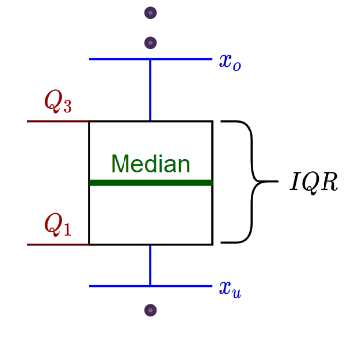
\includegraphics[width=\textwidth]{images/boxplot.png}
\end{minipage}
\end{definition}

\begin{KR}{Erstellen eines Boxplots}
\begin{enumerate}
    \item Berechne die Quartile $Q_1$, $Q_2$ (Median) und $Q_3$
    \item Bestimme den Interquartilsabstand IQR = $Q_3 - Q_1$
    \item Berechne die Grenzen für Ausreisser:
        \begin{itemize}
            \item Untere Grenze: $Q_1 - 1.5 \cdot IQR$ und Obere Grenze: $Q_3 + 1.5 \cdot IQR$
        \end{itemize}
    \item Zeichne Box mit:
        \begin{itemize}
            \item Unterer Rand bei $Q_1$, Mittelline bei $Q_2$, Oberer Rand bei $Q_3$
        \end{itemize}
    \item Zeichne Antennen bis zum:
        \begin{itemize}
            \item Kleinsten Wert  $\geqslant$  untere Grenze 
            \item Grössten Wert $\leqslant$  obere Grenze
        \end{itemize}
    \item Markiere alle Werte ausserhalb als Ausreisser
\end{enumerate}
\end{KR}

\begin{example2}{Boxplot - Praktisches Beispiel}
Messwerte: 2, 3, 5, 6, 7, 8, 9, 15, 50
\begin{enumerate}
    \item Sortiere Werte: 2, 3, 5, 6, 7, 8, 9, 15, 50
    \item Bestimme Quartile:
        \begin{itemize}
            \item $Q_1$ = 4 (25\%-Quantil), $Q_2$ = 7 (Median), $Q_3$ = 12 (75\%-Quantil)
        \end{itemize}
    \item IQR = 12 - 4 = 8
    \item Ausreisser-Grenzen:
        \begin{itemize}
            \item Untere: 4 - 1.5 · 8 = -8
            \item Obere: 12 + 1.5 · 8 = 24
        \end{itemize}
    \item 50 ist ein Ausreisser (> 24)
\end{enumerate}
\end{example2}

\raggedcolumns

\subsubsection{Lagekennwerte/Lageparameter}

\begin{concept}{Arithmetisches Mittel} $\bar{x}$ ist der Durchschnitt der Stichprobenwerte:

    \begin{minipage}{0.45\columnwidth}
        $$\bar{x} = \frac{1}{n}\sum_{i=1}^n x_i = \sum_{i=1}^m a_i \cdot f_i$$
    \end{minipage}
    \hspace{2mm}
    \begin{minipage}{0.5\columnwidth}
        \vspace{1mm}
        \begin{itemize}
            \item $a_i$: Klassenmitte
            \item $x_i$: Einzelner Stichprobenwert
            \item $f_i$: Relative Häufigkeit
        \end{itemize}
    \end{minipage}
\end{concept}

\begin{concept}{Median} Das 2. Quartil wird auch Median oder Zentralwert genannt:
    $$\text{Median}(x_1,...,x_n) = x_{\text{med}} = \begin{cases}
    x_{[\frac{n+1}{2}]} & \text{falls } n \text{ ungerade}\\
    \frac{1}{2}(x_{[\frac{n}{2}]} + x_{[\frac{n}{2}+1]}) & \text{falls } n \text{ gerade}
    \end{cases}$$
    teilt Datensatz in zwei gleich grosse Hälften
\end{concept}

\begin{concept}{Modus}
    $x_{mod}$ = Häufigster Wert in der Stichprobe
\end{concept}

\begin{remark}
\begin{itemize}
    \item Mittelwert reagiert empfindlich auf Ausreißer (A)
    \item Median ist robuster gegen Ausreißer
    \item Modus zeigt Häufungen, kann mehrfach auftreten
\end{itemize}
\end{remark}



\subsubsection{Streuungskennwerte}

\begin{remark}
\begin{itemize}
    \item $s$: Stichprobenstandardabweichung
    \item $s_{\text{kor}}$: Korrigierte Stichprobenstandardabweichung
    \item $s^2$: Stichprobenvarianz
    \item $s_{\text{kor}}^2$: Korrigierte Stichprobenvarianz
    \item $\bar{x}$: Arithmetisches Mittel
    \item $x_i$: Einzelner Stichprobenwert
\end{itemize}
\end{remark}

\begin{definition}{Streuungsmasse}\\
\textbf{Stichprobenvarianz:}
$$s^2 = \frac{1}{n}\sum_{i=1}^n (x_i - \bar{x})^2 = \frac{1}{n}\sum_{i=1}^n x_i^2 - \bar{x}^2 = \overline{x^{2}}-\bar{x}^{2}$$

\textbf{Korrigierte Stichprobenvarianz:}
$$s_{\text{kor}}^2 = \frac{1}{n-1}\sum_{i=1}^n (x_i - \bar{x})^2 = \frac{n}{n-1}s^2$$

\textbf{Standardabweichung:}
$$s = \sqrt{s^2} = \sqrt{\overline{x^{2}}-\bar{x}^{2}} \quad \text{bzw.} \quad s_{\text{kor}} = \sqrt{s_{\text{kor}}^2}$$
\end{definition}

\begin{KR}{Berechnung der Stichprobenvarianz}
\begin{enumerate}
    \item Berechne den Mittelwert $\bar{x}$
    \item Für jeden Wert $x_i$:
        \begin{enumerate}
            \item Berechne Abweichung vom Mittelwert $(x_i - \bar{x})$
            \item Quadriere die Abweichung $(x_i - \bar{x})^2$
        \end{enumerate}
    \item Summiere alle quadrierten Abweichungen
    \item Teile durch $(n-1)$ für korrigierte Varianz
    \item Alternative Berechnung:
        \begin{enumerate}
            \item Berechne $\overline{x^2}$ (Mittelwert der quadrierten Werte)
            \item Berechne $(\bar{x})^2$ (Quadrat des Mittelwerts)
            \item Varianz = $\overline{x^2} - (\bar{x})^2$
        \end{enumerate}
\end{enumerate}
\end{KR}

\begin{example2}{Berechnung von Varianz und Standardabweichung}\\
Gegeben sei die Datenreihe: 2, 4, 4, 6, 9
\vspace{2mm}\\
\textbf{Schritt 1:} Mittelwert berechnen:
$\bar{x} = \frac{2 + 4 + 4 + 6 + 9}{5} = 5$

\textbf{Schritt 2:} Abweichungen quadrieren:
\begin{center}
\begin{tabular}{|c|c|c|}
\hline
$x_i$ & $(x_i - \bar{x})$ & $(x_i - \bar{x})^2$ \\
\hline
2 & -3 & 9 \\
4 & -1 & 1 \\
4 & -1 & 1 \\
6 & 1 & 1 \\
9 & 4 & 16 \\
\hline
\end{tabular}
\end{center}

\textbf{Schritt 3:} Varianz berechnen:
$s_{\text{kor}}^2 = \frac{9 +1 + 1 + 1 + 16}{5-1} = \frac{28}{4} = 7$
\vspace{1mm}\\
\textbf{Schritt 4:} Standardabweichung berechnen:
$s_{\text{kor}} = \sqrt{7} \approx 2.65$
\vspace{2mm}\\
\textbf{Alternative Berechnung:}
\vspace{1mm}\\
\begin{itemize}
    \setlength{\itemsep}{1pt}
    \item $\overline{x^2} = \frac{4 + 16 + 16 + 36 + 81}{5} = 30.6$
    \item $(\bar{x})^2 = 5^2 = 25$
    \item $s^2 = 30.6 - 25 = 5.6$
    \item $s_{\text{kor}}^2 = \frac{5}{4} \cdot 5.6 = 7$
\end{itemize}
\end{example2}

\subsubsection{Form der Verteilung}

\begin{concept}{Verteilungsformen}
\begin{itemize}
    \item \textbf{Symmetrisch:} Rechte und linke Hälfte spiegelbildlich
    \item \textbf{Linkssteil (rechtsschief):}
    \begin{itemize}
        \item Daten links konzentriert
        \item $x_{\text{mod}} < x_{\text{med}} < \bar{x}$
    \end{itemize}
    \item \textbf{Rechtssteil (linksschief):}
    \begin{itemize}
        \item Daten rechts konzentriert
        \item $x_{\text{mod}} > x_{\text{med}} > \bar{x}$
    \end{itemize}
    \item \textbf{Modalität:}
    \begin{itemize}
        \item Unimodal: Ein Maximum
        \item Bimodal/Multimodal: Mehrere Maxima
    \end{itemize}
\end{itemize}
\end{concept}